\documentclass[english]{beamer} %\documentclass[naustrian]{beamer}

\usepackage{lmodern}
\usepackage[utf8]{inputenc}
\usepackage[T1]{fontenc}
\usepackage[naustrian]{babel}

\usepackage{pgfpages}
\usepackage[abs]{overpic}
\usepackage{skak}
%\usepackage{movie15}
\usepackage{graphicx}

\usepackage{pifont}
\newcommand{\cmark}{\ding{51}}
\newcommand{\xmark}{\ding{55}}
% Nützlich in Verbindung mit "dspdfviewer"
%\setbeameroption{show notes on second screen=right}

\usepackage{multimedia}
\usepackage{media9}

%\usepackage{graphicx}
\usepackage{listings} 
\usepackage{xcolor}
\usepackage{pdfpages}
\usepackage{amsmath}
\usepackage{fancyvrb}
\definecolor{mygrey}{rgb}{0.54,0.56,0.57}
\fvset{numbers=left,numbersep=2mm,frame=single,rulecolor=\color{mygrey},framesep=2mm,framerule=0.3mm,gobble=2}

\usepackage{listings}
\lstset{numbers=left,
				numberstyle=\tiny,
				numbersep=5pt,
	breaklines=true,
	showstringspaces=false,
	frame=l ,
	xleftmargin=15pt,
	xrightmargin=15pt,
	basicstyle=\ttfamily\scriptsize,
	stepnumber=1}

\setbeamertemplate{theorems}[numbered]

\usepackage{tikz}
\usetikzlibrary{tikzmark,fit}
\usepackage{textcomp} 

% % % % %


\makeatletter
\beamer@compresstrue
\makeatother

\useoutertheme[footline=authorinstitutetitle]{jku}
%\useouthertheme{jku}
\usecolortheme{jku}
\useinnertheme{jku}

\setbeamertemplate{navigation symbols}{}

\usepackage{graphicx}
\graphicspath{{./Layout/}}

\usepackage{pgf}

\usepackage{amsmath}

\author{Sophie Hofmanninger & Jan-Michael Holzinger}
\title{Solving Proximity Constraints}
\date{26.06.2019}
%\institute{Institute for Communications Engineering and RF-Systems}

\AtBeginSection{
  \ifnum\value{section}>1
    \begin{frame}
      \tableofcontents[currentsection]
    \end{frame}
  \fi
}


\AtBeginDocument{
  {
    \setbeamertemplate{headline}{%
      \begin{beamercolorbox}{section in head/foot}%
        \vskip2ex%
        \flushright%
        
\includegraphics[width=0.25\paperwidth]{jku}\hspace*{2ex}%
        \vskip2ex%
      \end{beamercolorbox}%
    }
    \setbeamertemplate{footline}{
      \raisebox{2ex}[0pt][0pt]{
%        \hskip1ex\includegraphics[height=2cm]{instituteCompact}%
      }
      ~\hfill
      \raisebox{4ex}[0pt][0pt]{
        \scriptsize
        \begin{tabular}{r}
          Johannes Kepler University, A-4040 Linz, Austria
        \end{tabular}
      }
    }
    
    \begin{frame}
      \titlepage
    \end{frame}
  }
}


% % % % %

\begin{document}
  \begin{frame}
    \tableofcontents
  \end{frame}
  
	\section{Introduction} \subsection{}

\begin{frame}[fragile=singleslide]
	\frametitle{Motivation}
		For proving theorems, a frequently occurring problem is to find common instances of formulae.
		\begin{exampleblock}{Example 1}
			Let \(f\) be a function, \(a,b\) constants and \(x\) a variable. The two expressions
			\[f(a,x)\quad\text{and}\quad f(a,b)\]
			can be unified with \(\{x\mapsto b\}\).
		\end{exampleblock}

  \end{frame}	
		
%---------------------------------------------------------------

\begin{frame}[fragile=singleslide]
	\frametitle{Motivation}
		For proving theorems, a frequently occurring problem is to find common instances of formulae.
		\begin{exampleblock}{Example 2}
			Let \(f,g\) be functions, \(a,b\) constants and \(x\) a variable. The two expressions
			\[f(a,x)\quad\text{and}\quad g(a,b)\]
			cannot be unified as \(f\neq g\).
		\end{exampleblock}

  \end{frame}	
		
%---------------------------------------------------------------
				
\begin{frame}[fragile=singleslide]
	\frametitle{Motivation}
		In 1965 Robinson presented his unification algorithm and solved this problem, his algorithm was improved for better(=faster) performance since.\\ \ \\
		If we consider now the unification problem \[f(a,x)\simeq^{?} g(a,b)\] again, we might wonder, if we could not ignore \(f\neq g\), if they are ``close'' to each other, i.e. if they are equal in a fuzzy logic sense.\\
		Being close is represented as a proximity relation, which are symmetric and reflexive, but not necessarily transitive. C. Pau and T. Kutsia solved this problem, presenting an algorithm, which we implemented.

  \end{frame}	
		
%---------------------------------------------------------------


	\begin{frame}[fragile=singleslide]
	\frametitle{Introduction}
		The Algorithm consists of two sub-algorithms and works on (modifies) 4 sets:
		\begin{itemize}
			\item P: unification problem to be solved ,
			\item C: neighbourhood constraint,
			\item $\sigma$: set of pre-unifier,
			\item $\Phi$: name-class mapping,
		\end{itemize}
		where Algorithm 1 modifies \(P,C,\) and \(\sigma\) and Algorithm 2 modifies \(C\) and \(\Phi\). If Algorithm 1 was successful, \(P=\emptyset\), if Algorithm 2 was successful \(C=\emptyset\). 
  \end{frame}	
		
%---------------------------------------------------------------
		
	\begin{frame}[fragile=singleslide]
	\frametitle{pre-Unification rules}
	\textcolor[rgb]{0.55,0,0}{(Tri)} \(\{x \simeq^? x\} \uplus P;C;\sigma \Rightarrow  P; C;\sigma\) \\
		\vspace{0.3cm}
		\textcolor[rgb]{0.55,0,0}{(Dec)} \(\{F(\overline{s_n}) \simeq^? G(\overline{t_n})\} \uplus  P;C;\sigma \Rightarrow \{\overline{s_n \simeq^?t_n}\}\cup P;\{F\approx^? G\}\cup  C;\sigma\) \\
		\vspace{0.3cm}
		\textcolor[rgb]{0.55,0,0}{(VE)} \(\{x \simeq^? t\} \uplus P;C;\sigma \Rightarrow  \{t'\simeq^? t\}\cup P{x\mapsto t'}; C;\sigma\{x\mapsto t'\}\) \\
		\vspace{0.3cm}
		\textcolor[rgb]{0.55,0,0}{(Ori)} \(\{t \simeq^? x\} \uplus P;C;\sigma \Rightarrow  \{x \simeq^? t\}\cup P; C;\sigma\) \\
		\vspace{0.3cm}
		\textcolor[rgb]{0.55,0,0}{(Cla)} \(\{F(\overline{s_n}) \simeq^? G(\overline{t_n})\} \uplus P;C;\sigma \Rightarrow  \bot\text{ if } m\neq n\) \\
		\vspace{0.3cm}
		\textcolor[rgb]{0.55,0,0}{(Occ)} \(\{x \simeq^? t\} \uplus P;C;\sigma \Rightarrow  \bot\text{ if there is an occurrence cycle of }x\text{ in }t\) \\
		\vspace{0.3cm}
		\textcolor[rgb]{0.55,0,0}{(VO)} \(\{x \simeq^? y, \overline{x_n\simeq^? y_n}\};C;\sigma \Rightarrow  \{\overline{x_n\simeq^? y_n}\}\{x\mapsto y\}; C;\sigma\{x\mapsto y\}\) \\
		\vspace{0.3cm}
	
  \end{frame}	
		
%---------------------------------------------------------------
		
		\begin{frame}[fragile=singleslide]
	\frametitle{Rules for Neighbourhood Constraints}
		\textcolor[rgb]{0.55,0,0}{(FFS)} $\{f \approx^? g\} \uplus C; \Phi \Rightarrow  C; \Phi; \text{ if } \mathcal{R}(f,g)\geq \lambda$ \\
		\vspace{0.3cm}
		\textcolor[rgb]{0.55,0,0}{(NFS)} $\{N \approx^? g\} \uplus C; \Phi \Rightarrow  C; update(\Phi,N\rightarrow \textbf{pc}(g,\mathcal{R},\lambda))$  \\
		\vspace{0.3cm}
		\textcolor[rgb]{0.55,0,0}{(FSN)} $\{g \approx^? N\} \uplus C; \Phi \Rightarrow  \{N \approx^? g\} \cup C;\Phi$  \\
		\vspace{0.3cm}
		\textcolor[rgb]{0.55,0,0}{(NN1)} $\{N \approx^? M\} \uplus C; \Phi \Rightarrow  C; update(\Phi,N\rightarrow \{f\}, M\rightarrow \textbf{pc}(f,\mathcal{R},\lambda))$, where $N \in dom(\Phi )$, $f\in \Phi(N)$ \\
		\vspace{0.3cm}
		\textcolor[rgb]{0.55,0,0}{(NN2)} $\{M \approx^? N\} \uplus C; \Phi \Rightarrow  \{N \approx^? M\} \cup C;\Phi$, where $M \notin dom(\Phi )$, $N\in dom(\Phi)$ \\
		\vspace{0.3cm}
		\textcolor[rgb]{0.55,0,0}{(Fail1)} $\{f \approx^? g\} \uplus C; \Phi \Rightarrow  \perp$, if $\mathcal{R}(f,g) < \lambda$ \\
		\vspace{0.3cm}
		\textcolor[rgb]{0.55,0,0}{(Fail2)} $C; \Phi \Rightarrow  \perp$, if there exists $N \in dom(\Phi )$ such that $\Phi (N)=\emptyset$ \\
		\vspace{0.3cm}
	
  \end{frame}	

%---------------------------------------------------------------

	\begin{frame}[fragile=singleslide]
	\frametitle{Simple example about how both algorithms work}
	\begin{exampleblock}{Example 3}
	Let $p,q$ and $f$ be functions, $b,c,c'$ constants and $x,z$ variables. Then the following unification problem has a solution:\\
	\[p(x,z) =^? q(f(b),f(x)) \quad \text{with}\quad R=\{(b,c'),(c',c),(p,q)\}\]\\
	\end{exampleblock}
	\end{frame}
	
%---------------------------------------------------------------
		% <presentation:0> to hide slide
		
		\begin{frame}<presentation:0>[fragile=singleslide]
	\frametitle{Simple example}
	\begin{exampleblock}{Example - both success}
	\(p(x,z) =^? q(f(b),f(x))\) and \(R=\{(b,c'),(c',c),(p,q)\}\)\\
	\end{exampleblock}
	\textbf{pre-Unification} \\
	
	\(P=\{p \simeq^? q\}\)\\
	\(C=\{\}\)\\
	\(\sigma=\{\}\)\\
	\(\Rightarrow^{\text{Dec}}\)\\
	\(P=\{x \simeq^? f, z \simeq^? f\}\)\\
	\(C=\{p \approx^? q\}\)\\
	\(\sigma=\{\}\)\\
	\(\Rightarrow^{\text{VE}}\)\\
	%\(P=\{N_1(N_2) \simeq^? f(b), z \simeq^? f(N_1(N_2))\}\)\\
	%\(C=\{p \approx^? q\}\)\\
	%\(\sigma=\{x \mapsto N_1(N_2)\}\)\\
	%\(\Rightarrow^{\text{Dec}^2}\)\\
	
	\end{frame}
	\begin{frame}<presentation:0>[fragile=singleslide]
	\frametitle{Simple example cont.}
	\(P=\{N_1(N_2) \simeq^? f(b), z \simeq^? f(N_1(N_2))\}\)\\
	\(C=\{p \approx^? q\}\)\\
	\(\sigma=\{x \mapsto N_1(N_2)\}\)\\
	\(\Rightarrow^{\text{Dec}^2}\)\\
	\(p(x,z) =^? q(f(b),f(x)) ; R=\{(a,a'),(a',b),(b,c'),(c',c),(p,q)\}\)\\
	\(P=\{z \simeq^? f\}\)\\
	\(C=\{p \approx^? q, N_1 \approx^? f, N_2 \approx^? b\}\)\\
	\(\sigma=\{x \mapsto N_1(N_2)\}\)\\
	\(\Rightarrow^{\text{VE}}\)\\
	\(P=\{N_3(N_4(N_5)) \simeq^? f(N_1(N_2))\}\)\\
	\(C=\{p \approx^? q, N_1 \approx^? f, N_2 \approx^? b\}\)\\
	\(\sigma=\{x \mapsto N_1(N_2),z \mapsto N_3(N_4(N_5))\}\)\\
	\(\Rightarrow^{\text{Dec}^3}\)\\
	\end{frame}
	
	\begin{frame}<presentation:0>[fragile=singleslide]
	\frametitle{Simple example cont.}
	\(P=\{\}\)\\
	\(C=\{p \approx^? q, N_1 \approx^? f, N_2 \approx^? b, N_3 \approx^? f, N_4 \approx^? N_1, N_5 \approx^? N_2\}\)\\
	\(\sigma=\{x \mapsto N_1(N_2), z \mapsto N_3(N_4(N_5))\}\)\\
	
	\vspace{0.5cm}
	\textbf{Constraint Simplification}\\
	\(C=\{p \approx^? q, N_1 \approx^? f, N_2 \approx^? b, N_3 \approx^? f, N_4 \approx^? N_1, N_5 \approx^? N_2\}\)\\
	\(\Phi=\{\}\)\\
	\(\Rightarrow^{\text{FFS}}\)\\
	\(C=\{N_1 \approx^? f, N_2 \approx^? b, N_3 \approx^? f, N_4 \approx^? N_1, N_5 \approx^? N_2\}\)\\
	\(\Phi=\{\}\)\\
	\(\Rightarrow^{\text{NFS}^3}\)\\
		\end{frame}
		
		\begin{frame}<presentation:0>[fragile=singleslide]
	\frametitle{Simple example cont.}
	
	\textcolor[rgb]{0,0.58,0}{\begin{flushright}
	\(R=\{(b,c'),(c',c),(p,q)\}\)
	\end{flushright}}
	\(C=\{N_4 \approx^? N_1, N_5 \approx^? N_2\}\)\\
	\(\Phi=\{N1\mapsto \{f\}, N2\mapsto \{b,c'\}, N3\mapsto \{f\} \}\)\\
	\(\Rightarrow^{\text{NN2}}\)\\
	\(C=\{N_1 \approx^? N_4, N_5 \approx^? N_2\}\)\\
	\(\Phi=\{N1\mapsto \{f\}, N2\mapsto \{b,c'\}, N3\mapsto \{f\} \}\)\\
	\(\Rightarrow^{\text{NN1}}\)\\
	\(C=\{N_5 \approx^? N_2\}\)\\
	\(\Phi=\{N1\mapsto \{f\}, N2\mapsto \{b,c'\}, N3\mapsto \{f\} , N4\mapsto \{f\}\}\)\\
	\(\Rightarrow^{\text{NN2,NN1}}\)\\
		\end{frame}
		
		\begin{frame}<presentation:0>[fragile=singleslide]
	\frametitle{Simple example cont.}
	\(C=\{\}\)\\
	\(\Phi_1=\{N1\mapsto \{f\}, N2\mapsto \{b\}, N3\mapsto \{f\} , N4\mapsto \{f\},N5\mapsto \{b,c'\}\}\)\\
	\(\Phi_2=\{N1\mapsto \{f\}, N2\mapsto \{c'\}, N3\mapsto \{f\} , N4\mapsto \{f\},N5\mapsto \{b,c',c\}\}\)\\
	
	\vspace{0.5cm}
	\textbf{Solution}\\
	\(\Phi_1=\{N1\mapsto \{f\}, N2\mapsto \{b\}, N3\mapsto \{f\} , N4\mapsto \{f\},N5\mapsto \{b,c'\}\}\)\\
	\(\Phi_2=\{N1\mapsto \{f\}, N2\mapsto \{c'\}, N3\mapsto \{f\} , N4\mapsto \{f\},N5\mapsto \{b,c',c\}\}\)\\
	\(\sigma=\{x \mapsto N_1(N_2), z \mapsto N_3(N_4(N_5))\}\)\\
		\end{frame}
		%---------------------------------------------------------------
		
	\begin{frame}[fragile=singleslide]
	\frametitle{Simple example - pre-Unification fails}
	\begin{exampleblock}{Example [Fail pU] }
	Examples where the pre-Unification algorithm fails:
		\begin{gather}
		\begin{align}
				\text{\textcolor[rgb]{0,0.58,0}{(Occ)}}\quad & p(x) =^? q(f(x))\\
				\text{\textcolor[rgb]{0,0.58,0}{(Cla)}}\quad & p(a,b) =^? q(f(x))
		\end{align}
		\end{gather}
	\end{exampleblock}
		\vspace{0.5cm}
		\end{frame}
	
	\begin{frame}[fragile=singleslide]
	\frametitle{Simple example - Constraint Simplification fails}		
	\begin{exampleblock}{Example [Fail CS]}
	Let $p$ and $q$ be functions, $a,b,c$ constants and $x,y$ variables. Then for the following unification problem only the pre-Unification algorithm is successful:
	\[p(a,x,a) =^? q(y,b,x) \quad \text{with} \quad R=\{(b,c),(p,q)\}\]\\
	\end{exampleblock}
	\end{frame}
	
	\begin{frame}[fragile=singleslide]
	\frametitle{Simple example cont.}
	\textbf{pre-Unification}\\
	\ldots \\
	\(C=\{p \approx^? q, N_1 \approx^? a, N_2 \approx^? b, a \approx^? N_2\}\)\\
	
	\vspace{0.5cm}
	\textbf{Constraint Simplification}\\
	\(C=\{p \approx^? q, N_1 \approx^? a, N_2 \approx^? b, a \approx^? N_2\}\)\\
	\(\Phi=\{\}\)\\
	\(\Rightarrow^{\text{FFS}}\)\\
	\(C=\{N_1 \approx^? a, N_2 \approx^? b, a \approx^? N_2\}\)\\
	\(\Phi=\{\}\)\\
	\(\Rightarrow^{\text{NFS}^2}\)\\
  \end{frame}	
	
	\begin{frame}[fragile=singleslide]
	\frametitle{Simple example cont.}
	\(C=\{ a \approx^? N_2\}\)\\
	\(\Phi=\{N_1\mapsto \{a\}, N_2\mapsto \{b,c\}\}\)\\
	\(\Rightarrow^{\text{FSN}}\)\\
	\(C=\{ N_2 \approx^? a\}\)\\
	\(\Phi=\{N_1\mapsto \{a\}, N_2\mapsto \{b,c\}\}\)\\
	\(\Rightarrow^{\text{NFS}}\)\\
	\(C=\{\}\)\\
	\(\Phi=\{N_1\mapsto \{a\}, N_2\mapsto \emptyset\}\)\\
	\(\Rightarrow^{\text{Fail2}}\)\\
	\(\perp\)
  \end{frame}

	\section{System Model} \subsection{}
	
	\begin{frame}[fragile=singleslide]
	\frametitle{System Model}
	 
	Project consists of 4 packages:
		\begin{itemize}
			\item elements : contains all needed types
			\item tool : offers important tools (e.g. store proximity relations)
			\item unificationProblem : has the core features
			\item userInterfaces : provide user interfaces
		\end{itemize}
	
  \end{frame}	
		
%---------------------------------------------------------------

	\begin{frame}[fragile=singleslide]
	\frametitle{Package \texttt{elements}}
	
	\begin{figure}
		\centering
			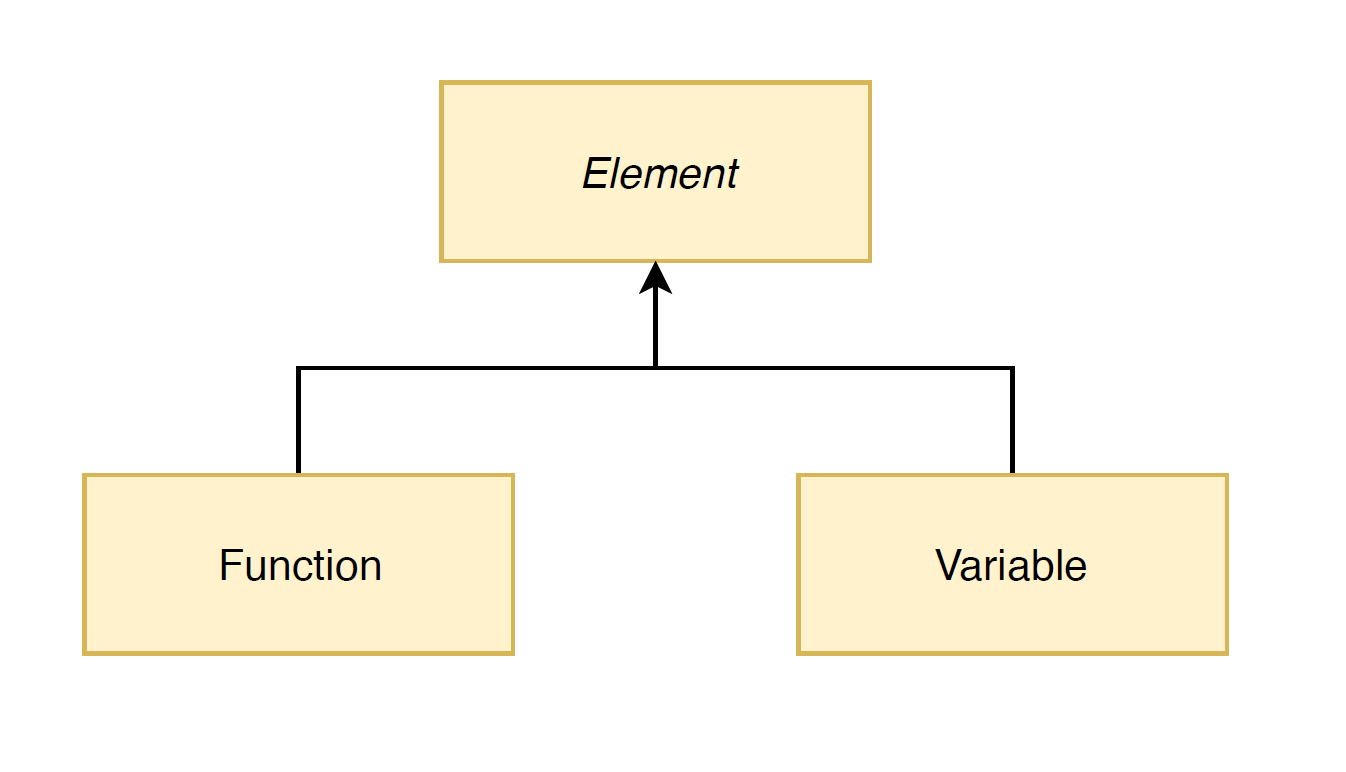
\includegraphics[width=8cm]{Bilder/elements.PNG}
		\label{fig:elements}
	\end{figure}
	
  \end{frame}	

%---------------------------------------------------------------

	\begin{frame}[fragile=singleslide]
	\frametitle{Package \texttt{tool}}
	 
	\begin{figure}
		\centering
			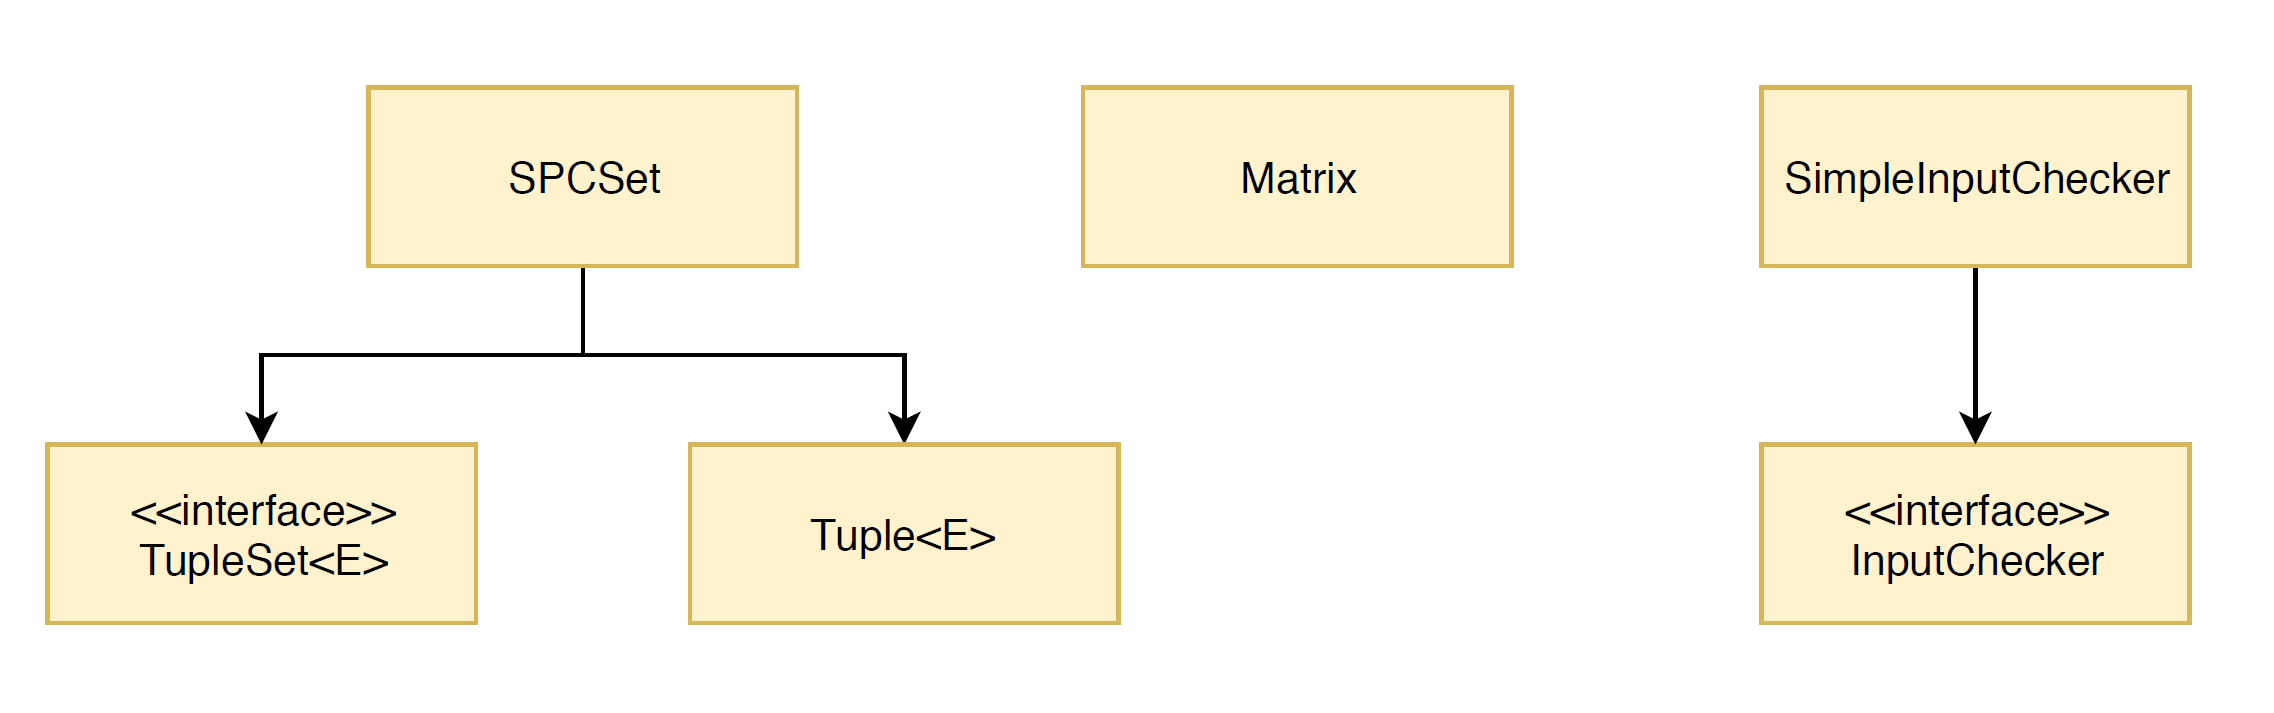
\includegraphics[width=11cm]{Bilder/tool.PNG}
		\label{fig:tool}
	\end{figure}
	
  \end{frame}	

%---------------------------------------------------------------

	\begin{frame}[fragile=singleslide]
	\frametitle{Package \texttt{unificationProblem}}
	 
	\begin{figure}
		\centering
			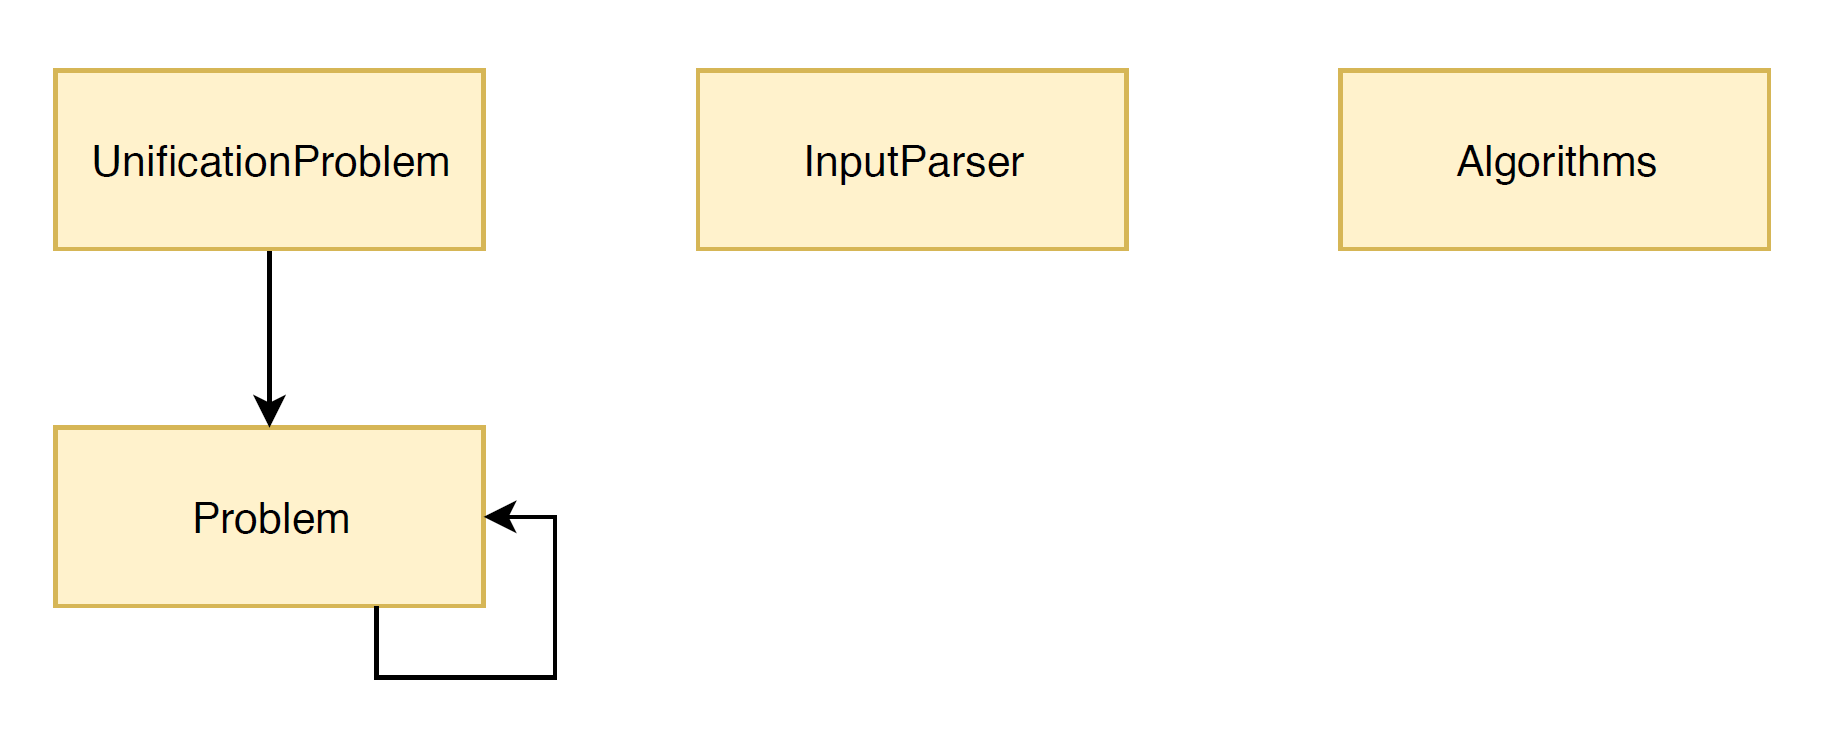
\includegraphics[width=11cm]{Bilder/unificationProblem.PNG}
		\label{fig:uP}
	\end{figure}
	
  \end{frame}	
	
%---------------------------------------------------------------
	
	\begin{frame}[fragile=singleslide]
	\frametitle{Package \texttt{userInterfaces}}
	 
	\begin{figure}
		\centering
			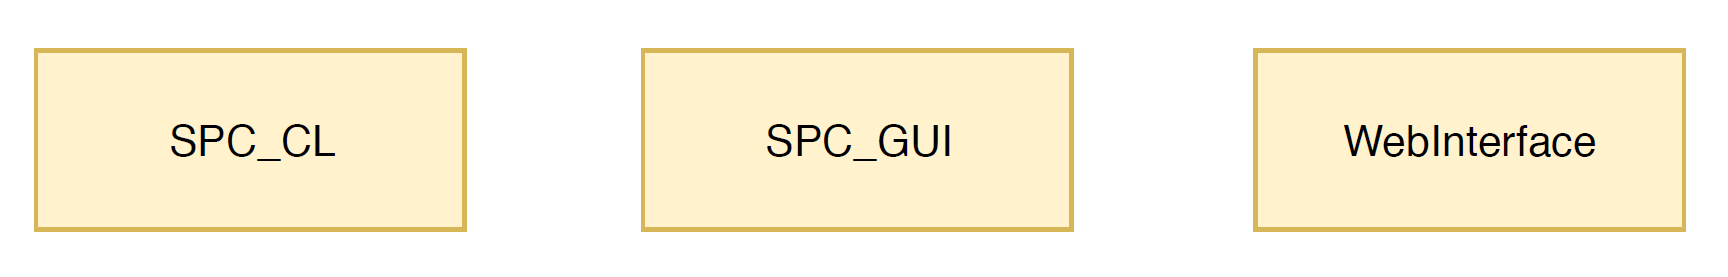
\includegraphics[width=11cm]{Bilder/userInterfaces.PNG}
		\label{fig:uI}
	\end{figure}
	
  \end{frame}

%===============================================================
	\section{Workflow} \subsection{}
%===============================================================
	
		\begin{frame}[fragile=singleslide]
		\frametitle{Workflow}
		
		\begin{figure}
			\centering
				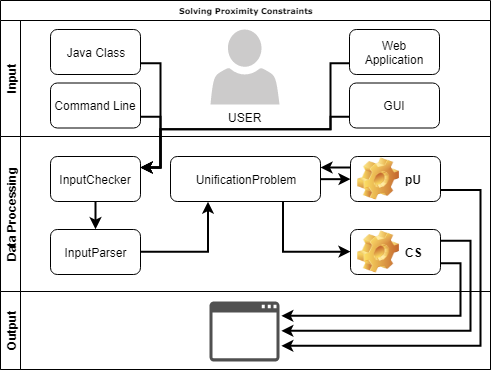
\includegraphics[width=8cm]{Bilder/WorkFlow.PNG}
			\label{fig:WorkFlow}
		\end{figure}
		
		\end{frame}

%---------------------------------------------------------------

	\section{Usage and Experience with the presented Tools} 
\begin{frame}[fragile=singleslide]
	\frametitle{Redmine}
	We found Redmine and its features very helpful for Software development. Mainly, we used it to keep track of work that has to be done, that was done, and also see what the other person is working on. We also tried out the Forum, to communicate when we needed, but we found Whatsapp more suitable for this.\\
	For communication: In our opinion, communication is one of the most important things when working in a team, but we tried to restrict ourselves to the communications channels offered by the lecture, so basically Redmine, meeting a few minutes before the lecture, and Whatsapp that is like the Forum + notification when read.
  \end{frame}
	
	%---------------------------------------------------------------
	\begin{frame}[fragile=singleslide]
		\frametitle{Git/Javadoc}
	As it is a requirement for the project, we of course used git alot. We tried to use branches and merge. As suggested, we committed (and most of the times also pushed) as soon as we further developed the project. As we did not work on the project for 8 hours straight every day in the week, this pretty much models the usage in a company, where you pull at the beginning, then work/commit to save your work and at the end of the day (or at a ``milestone'') push.\\
	It was very important to us to use Javadoc from the beginning on for almost each method. The reason for that was that eclipse has the nice feature of displaying it as a tooltip, and so you can understand easily the behaviour of the method, even if the other person implemented it.
  \end{frame}
	
	%---------------------------------------------------------------
	\begin{frame}[fragile=singleslide]
			\frametitle{JUnit/Jenkins}
	For testing, that was very necessary, to find bugs, we used JUnit 5, although we later found out it is not too easy to use it from command line/Jenkins. It also was a good feeling, that whenever one had altered parts of the code, and run JUnit everything worked out again. At the beginning we had the feeling that Jenkins would not be as useful in our project as it might be in others, but actually, it was nice to use it to simply run all tests. Even though realizing that JUnit 5 has (also) strict naming conventions for test classes took us some time.
  \end{frame}
%---------------------------------------------------------------
		%\begin{frame}
		%\huge{Thank you for your attention.}
	  %\end{frame}
%---------------------------------------------------------------

\end{document}